\chapter{Random Circuit Sampling}
\label{sec:rcs}

Despite four decades
of research in quantum computing, 
there was no physical proof of whether it would be possible to realize quantum computers
that have an advantage over classical ones. This only changed
recently, when a team from Google and the UCSB claimed to have demonstrated \textit{quantum supremacy}
with a 54 superconducting qubit quantum processor \cite{martines2019supremacy}. For this purpose, they
chose the problem of \textit{random circuit sampling}, a problem designed explicitly
as a quantum supremacy experiment \cite{Boixo2018supremacy}.

This chapter will motivate and introduce the theoretical framework of random circuit
sampling, also used as the benchmark for restricted Boltzmann machines in this
study. Further, the results of Google's quantum supremacy experiments will be discussed.

\section{Quantum Supremacy}
\label{sec:quantum_supremacy}

John Preskill has coined the term \textit{quantum supremacy} in 2012
\cite{preskill2012quantum}. It describes the point in time when a physical quantum computer
outperforms a classical computer on some task for the first time. The problem
solved by the quantum computer does not need to be useful. Its only purpose is
to prove that a quantum computer can be realized which has an advantage over
classical computers on \textit{some} problem.

There exist different proposals for quantum supremacy
experiments \cite{shor1997factorisation, aaronson2013boson, Boixo2018supremacy}. Since quantum computers do not promise to outperform classical
computers on every problem, as discussed in section~\ref{sec:quantum_computational_complexity}, 
quantum supremacy experiments must be based upon a strong theoretical foundation \cite{Bernstein93quantumcomplexity}.

One way to demonstrate quantum supremacy would be to run Shor's
algorithm for integer factorization \cite{shor1997factorisation} on a physical quantum computer on some number which would not be feasible
to decompose with known classical algorithms on existing supercomputers \cite{martinlopez2011experimental}. 
For this approach, about 10,000 error-corrected qubits with full connectivity are necessary to factorize current 
RSA keys with a length of 2048 bits \cite{Barker15nistspecial,shor1997factorisation}. Today it is possible to
build quantum processors with merely about 50 noisy qubits of reasonable quality and restricted connectivity \cite{martines2019supremacy}.

Another famous proposal for a quantum supremacy experiment is \textit{Boson Sampling} \cite{aaronson2013boson}, which is based on the
fact that calculating the permanent of a matrix is computationally hard. This experiment requires less 
physical resources than necessary for a full quantum computing setup. A special case of 
Boson Sampling is Gaussian Boson Sampling, which has been co-developed by researchers 
from the University of Paderborn, Germany \cite{Hamilton2017}. In Gaussian Boson Sampling, squeezed states are injected 
into every input mode, instead of applying single photons as in the case of standard 
boson sampling.

Instantaneous quantum polynomial-time (IQP) quantum circuits are a third candidate to demonstrate 
quantum supremacy. Such circuits are provable hard to simulate classically, even in the presence of 
noise \cite{Bremner2017}.

The approach that a team from Google and UCSB took last year is called \textit{Random
  Circuit Sampling} (RCS) \cite{Boixo2018supremacy, martines2019supremacy}. In this approach, random quantum circuits of specific structures that create highly
entangled states are run on a quantum processor and are simulated classically. For
enough qubits and depth, performing the classical simulations would take years on the biggest 
existing supercomputers, according to Google \cite{martines2019supremacy}. If the quantum computer can generate outputs
for such circuits which cannot be simulated classically anymore while their output can still be
verified to be correct, this would demonstrate quantum supremacy. 

A metric that
allows the verification on random circuit instances that cannot be simulated is
the \textit{cross entropy difference}.

\section{Cross Entropy Difference}
\label{sec:cross_entropy}

The challenge of quantum supremacy is that one has to be able to verify the
results of the quantum computer on instances which cannot be calculated
classically anymore. In the case of integer factorization, this is a simple task
as the test for the correctness consists of simple multiplications which can be
performed efficiently. Since integer factorization needs more qubits than
currently available in existing quantum computer hardware, other supremacy
experiments like RCS provide a framework to demonstrate quantum supremacy much
earlier.

The first observation to understand the concept of RCS is that every quantum
circuit acting on $n$ qubits can be described by a single $2^n$ dimensional
unitary matrix \cite{nielsen2002quantum}, as illustrated in figure~\ref{fig:circuitasunitary}. This follows
from the fact that quantum gates are described by unitary transformations.
The matrix product, as well as the tensor product of two unitaries is a unitary again.

\begin{figure}[H]
  \begin{equation}
      \vcenter{
          \Qcircuit @C=1em @R=1em {
          & \ctrl{2} & \qw & \gate{H} & \ctrl{1} &
          \gate{H} & \qw \\
          & \qw & \ctrl{1} & \gate{H} & \targ &
          \gate{H} & \qw \\
          & \targ & \targ & \gate{Z} & \qw & \ctrl{-1} &
          \qw
        }
      }
      =
      \vcenter{
        \Qcircuit @C=1em @R=0em {
          & \multigate{2}{U} & \qw \\
          & \ghost{U} & \qw \\
          & \ghost{U} & \qw
        } 
      }
    \end{equation}
  \caption[Quantum Circuits as Unitaries]{Every Circuit can be described by one big unitary acting on $n$
    qubits. W.l.o.g. the resulting states correspond to the first column of the
    unitary $U$, assuming the circuit is initialized in the $\Ket{0}^{\otimes{n}}$ state.}
    \label{fig:circuitasunitary}
\end{figure}

A quantum circuit consisting of gates chosen uniformly at random
will act like a uniformly random unitary $U$ \cite{Boixo2018supremacy}. Since the input state of the circuit can be assumed to be
initialized in the $\Ket{0}^{\otimes n}$ state, the amplitudes of the final
quantum state of the circuit can be assumed to correspond to the first column of the random unitary $U$.

The distribution of universal random quantum circuits converges to the uniform (Haar) measure with increasing depth \cite{Emerson_2003}. 
This implies that the column's entries are complex numbers with real and imaginary parts
distributed by an unbiased Gaussian with respect to the normalization constraints.
The output probabilities of the random circuit are given by
the squared norms of these entries.
They are thus distributed as the square of
a Gaussian, which is an exponential distribution,
also known as a Porter-Thomas distribution \cite{Porter1956Fluctuations}. The normalized probabilities $p_j := p(x_j) =
| \Braket{x_j | \psi_{RC}} | ^2$ to observe bitstrings $x_j \in \{0,1\}^n$
are distributed according to

\begin{equation}
  Pr(Np_j) = e^{-Np_j}
\end{equation}

with $N=2^n$. The shape of this distribution is visualized in figure~\ref{fig:porterthomas}.

\begin{figure}[H]
  \centering
  \begin{tikzpicture}
    \begin{axis}[
      xmin=0,
      ymin=0,
      xmax=1,
      ymax=1,
      xlabel={$Np_j$},
      ylabel={$Pr(Np_j)$},
      xticklabels={},
      yticklabels={}
      ]
      \addplot[blue, domain=0:1, thick] {e^(-5*(1-x))};
    \end{axis}
  \end{tikzpicture}
  \caption[Output Distribution of Random Quantum Circuits]{Shape of the distribution $Pr(Np_j)$ of normalized output probabilities $Np_j$ of a
    random quantum circuit. The distribution $Pr(Np_j)=e^{-Np_j}$ is distributed as
    Porter-Thomas. A lot of output strings will have a low probability to be
    observed and a few output strings will dominate the observed outputs \cite{Boixo2018supremacy}.}
  \label{fig:porterthomas}
\end{figure}

As quantum computers suffer from decoherent noise \cite{Zeh:1970zz}, it is
important to understand if noisy quantum computers can still
outperform classical computers on the RCS task. Knowing that the outputs are
Porter-Thomas distributed will help with that.

The task is to understand how samples $S=\{x_1,\dots,x_m\}$ drawn from a perfect execution of
$U$ compare to a set $S^{\prime}=\{x_1^{\prime},\dots,x_m^{\prime}\}$ of samples drawn from a potentially noisy
execution of $U$.

Ideally, all output probabilities of the whole state space would be available. In that case, 
the total variation distance (TVD) could measure the closeness of the perfect and the potentially noisy 
execution. Unfortunately, for quantum circuits in the supremacy regime, the state space is too big 
to calculate this metric. Additionally, the amplitudes cannot be accessed directly in a quantum computer. 
A double exponential number of measurements would be necessary to estimate all outcome probabilities.
On a subset of the whole state space, the TVD could only ever proof that the two distributions are apart, but 
could not show closeness of the two. 
This makes it impossible to use the TVD to measure the accuracy of the execution of a quantum circuit.

Another measure for the similarity of two probability distributions is the \textit{cross entropy} \cite{kullback1951}.
It is equivalent to the negative of the log likelihood of the two distributions.
The cross entropy of the underlying
probability distributions $p_U$ and $p_U^{\prime}$ of samples taken from $S$ and $S^{\prime}$ respectively, is

\begin{equation}
  H(p_U^{\prime},p_U) = - \sum_{j=1}^Np_U^{\prime}(x_j|U) \log{p_U(x_j)},
\end{equation}

where $p_U^{\prime}(x_j|U)$ denotes the probability of $x_j$ in a noisy execution of circuit $U$.

Of interest is the expected quality of the potentially noisy execution over
different random circuit instances:

\begin{align}
  \label{eq:expectedCrossDifference}
  \mathbb{E}_U[H(p_U^{\prime},p_U)] &= \mathbb{E} \left[\sum_{j=1}^Np_U^{\prime}(x_j|U)\log{\frac{1}{p_U(x_j)}}\right]
\end{align}

The output of a worst-case (polynomial-time classical) noisy execution can be assumed to
be statistically uncorrelated with the output of the perfect execution \cite{Boixo2018supremacy}. 
For independent probability distributions $A$ and $B$, $\mathbb{E}[AB] = \mathbb{E}[A] \mathbb{E}[B]$. Thus,
and since the output distribution for a fixed $x_j$ over many random circuit
instances $U$ also has the shape of the Porter-Thomas distribution \cite{harrow2008random},
$\mathbb{E}_U[\log{\frac{1}{p_U(x_j)}}] = -\mathbb{E}_U[\log{p_U(x_j)}]$ from equation~\ref{eq:expectedCrossDifference} 
in this case can be computed as:

\begin{align}
  -\mathbb{E}_U[\log{p_U(x_j)}] &\approx - \int_0^{\infty}Ne^{-Np}\log{p} \,dp \\
                                &= \log{N} + \gamma,
\end{align}

where $\gamma \approx 0.577$ is the Euler constant.
Using the fact that $\sum_{j=1}^Np_U^{\prime}(x_j) = 1$ for any distribution $p_U{\prime}$, the average cross
entropy $\mathbb{E_U}[H(p_U^{\prime},p_U)]$ between the Porter-Thomas distribution and any other uncorrelated distribution is
given as 

\begin{equation}
  \mathbb{E}_U [H(p_U^{\prime},p_U)] = \log{N} + \gamma.
\end{equation}

This is equivalent to the cross entropy $H_0 = \log{N} + \gamma$ between the
Porter-Thomas and the uniform distribution. Thus, on
average, a worst-case noisy execution will be as good compared to a perfect execution as sampling
every bitstring with probability $1/N$. $H_0$ differs from the entropy $H(p_U)$ of
the Porter-Thomas distribution, which corresponds to the cross entropy with
itself, only by a $-1$ term:

\begin{align}
  H(p_U) &= - \int p N^2e^{-Np}\log{p} \, dp \\
         &= \log{N} -1 + \gamma,
\end{align}

This directly leads to a benchmark for any algorithm $A_U$ sampling output strings from a
random circuit $U$, given either by a
classical simulation or by a (noisy) quantum computer. The quality of 
$A_U$ can be calculated as the difference between
the entropy of the uniform distribution and the cross entropy of the output
samples from $A_U$ with the Porter-Thomas distribution. This metric is
defined as the \textit{cross entropy difference} \cite{Boixo2018supremacy}:

\begin{align}
  \Delta H(p_A) &\equiv H_0 - H(p_A, p_U) \\
                 &=\sum_j \left(\frac{1}{N} - p_A(x_j|U)\right)\log{\frac{1}{p_U(x_j)}}.
\end{align}

The cross entropy difference is zero for an algorithm sampling from the uniform
distribution and one for an algorithm sampling from the underlying Porter-Thomas
distribution of the circuit.

As shown shortly, the cross entropy difference can be estimated with a constant 
number of samples, independent of the number of qubits. It interpolates between 
a worst case (uniform random) and a perfect execution (Porter-Thomas) and assumes 
a decoherent noise channel in the execution of the quantum circuit. 
The cross entropy difference is related to the TVD by Pinsker's inequality. Nevertheless, 
a high cross entropy difference does not automatically imply a low TVD \cite{bouland2018quantum}.

In order to calculate $\Delta H(p_A)$, 
a perfect simulation of the random circuit is necessary as the values of $p_U(x_j)$ have to be known. This is not possible in the quantum
supremacy regime. As discussed shortly, it will be possible
to extrapolate the cross entropy difference $\Delta H(p_A)$ of $A_U$ to the quantum supremacy regime with high
precision based on samples of its cross entropy difference on smaller circuit
instances which can still be simulated classically \cite{Boixo2018supremacy}.

Another justification for the cross entropy difference is that the $l_1$ distance between the uniform distribution $p$ and Porter-Thomas distribution $q$

\begin{align}
  l_1(p,q) &= \| p-q\|_1 \\
           &= \sum_{j=1}^N \mid p_i - q_i \mid \\
           &= \frac{2}{e}
\end{align}

and thus independent of the number of qubits $n$. Therefore, a
constant number of samples is sufficient to calculate the cross entropy difference $H(p_U)$.

Experimentally, the cross entropy difference

\begin{equation}
  \alpha = \mathbb{E}_U[\Delta H(p^{\prime}_U)]
\end{equation}

can be obtained by the execution of several random circuits $U$. Quantum
supremacy is achieved by a physical quantum computer when its average cross
entropy

\begin{equation}
  1 \geq \alpha > C
\end{equation}

is greater than the average performance $C$ of the best known classical algorithm $A^*$ with 
output distribution $p^*$:

\begin{equation}
  C = \mathbb{E}_U[\Delta H(p^*)] .
\end{equation}

In the regime where perfect simulations are possible, $C=1$ and quantum
supremacy cannot be achieved \cite{Boixo2018supremacy}. For sufficiently many qubits, perfect simulations
will not be possible anymore and $1 > C \geq 0$ with $C$ decreasing exponentially
with the number of gates $g\gg n$. For a typical set of samples $S_{exp} = \{x_1^{exp}, \dots , x_m^{exp}\}$ drawn from the
execution of a quantum circuit, the central limit theorem implies that:

\begin{equation}
  \label{eq:cef}
  \alpha \simeq H_0 - \frac{1}{m} \sum_{j = 1}^m \log{\frac{1}{p_U(x_j^{exp})}}.
\end{equation}

The experimental setup to estimate the cross entropy difference of any
approximate simulation of a quantum computer thus is \cite{Boixo2018supremacy}:

\begin{enumerate}
\item Select random circuit $U$.
  \item Take sufficiently many samples $S_{exp} = \{x_1, \dots, x_m\}$, m in
    range $10^3-10^6$.
    \item Compute the quantities $\log{\frac{1}{p_U(x_j^{exp})}}$ with the aid
      of a sufficiently large classical computer.
      \item estimate $\alpha$ using equation~\ref{eq:cef}.
\end{enumerate}

\section{Extrapolating to the Supremacy Regime}
\label{sec:supremacy_regime}

Keeping the qubits in a coherent state during a calculation and applying quantum
gates exactly is a difficult task \cite{martines2019supremacy}. Qubits will suffer from decoherent noise, which will destroy the quantum states. This will happen in particular in the early implementations of quantum computers.

Before large scale error-corrected quantum computers become available, so-called noisy intermediate-scale quantum (NISQ) computers present the first stage
of quantum computing hardware. Such noisy devices will already provide an
advantage over classical computers on specific problems. If the noise can be
kept below a certain threshold, a NISQ device can demonstrate quantum
supremacy on the RCS task \cite{neill2018blueprint}.

In the presence of noise, the quantum state $\rho$, also called the density operator, generated by a physical quantum computer
after the execution of a random circuit $U$ can be represented as

\begin{equation}
  \rho = \tilde{\alpha} U \Ket{\psi_0} \Bra{\psi_0} U^{\dagger} + (1- \tilde{\alpha}) \sigma
\end{equation}

with $\tilde{\alpha}$ being the circuit \textit{fidelity} and noise term $\sigma$ being an orthogonal mixed state to the true state with
$\Bra{\psi_0}U^{\dagger}\sigma U \Ket{\psi_0} = 0$.
The corresponding average cross entropy difference is:

\begin{align}
  \alpha &= \mathbb{E}_U\left[H_0+ \sum_j \Bra{x_j} \rho \Ket{x_j} \log{p_U(x_j)} \right] \\
         &= \tilde{\alpha} + (1-\tilde{\alpha})H_0 + \mathbb{E}_U\left[(1-\tilde{\alpha}) \sum_j \Bra{x_j} \sigma \Ket{x_j} \log{p_U(x_j)}\right].
\end{align}

The states generated by the random circuits are
maximally entangled \cite{Boixo2018supremacy}. A single bit or phase flip introduced by an additional $ X $ or $ Z $ gate in the circuit completely destroys such a state. Instead of being Porter-Thomas distributed, the output would be almost uniformly distributed, as shown in figure~\ref{fig:rcs_noise}.

\begin{figure}[H]
  \centering
  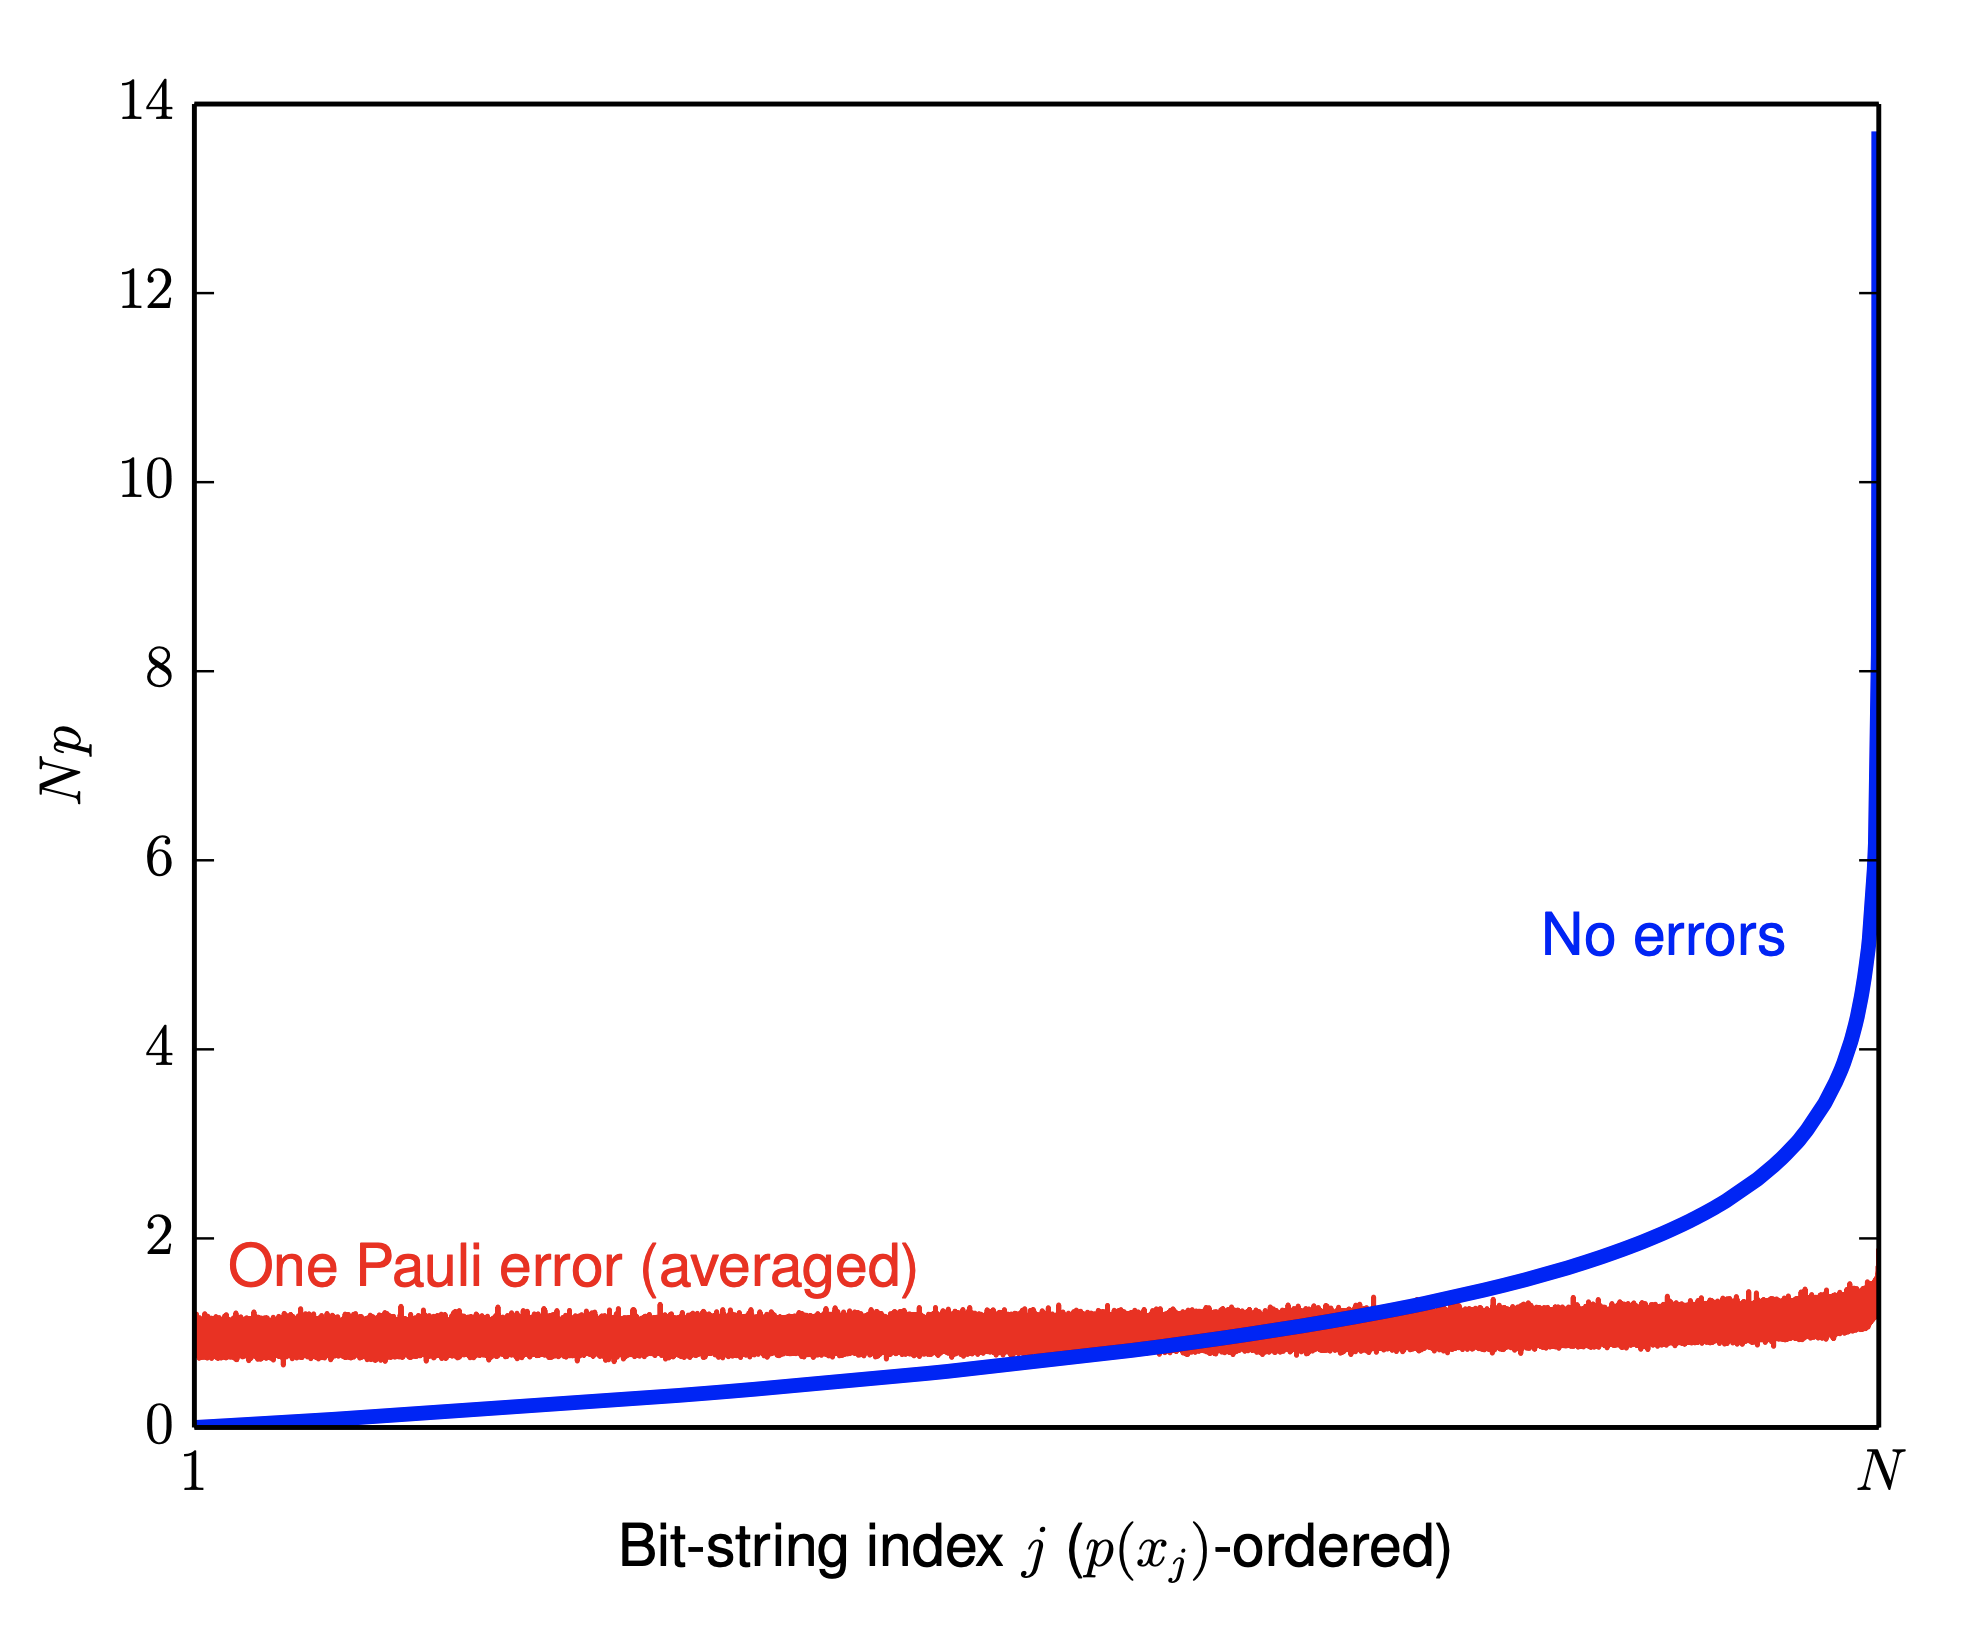
\includegraphics[width=0.58\textwidth]{figures/rcs_noise}
  \caption[Effect of One Pauli-Error on Random Circuits]{Blue ("No errors"): Output bitstrings of a random circuit ordered by their probabilities. Red ("One Pauli error"): Averaged 
  simulated output distribution with one Pauli-error on all possible positions in a $5 \times 4$ qubits random circuit 
  with depth 40. The distribution is almost uniform and almost uncorrelated with the real output distribution. The small tilt at 
  the end can be explained by the fact that Z gates close to the end of the circuit do not have an effect on the output distribution. Figure taken from \cite{Boixo2018supremacy}.}
  \label{fig:rcs_noise}
\end{figure}

In other words, it is not possible to infer any information about the output
probabilities without a perfect simulation of the circuit.
This justifies the assumption that the actual output probabilities and the output
of the quantum computer are (almost) uncorrelated.
This assumption of no correlation, in turn, leads to the conclusion that the
circuit fidelity $\tilde{\alpha}$ of a random
circuit $U$ is approximately equal to the average cross entropy:

\begin{equation}
  \label{eq:extrapolate}
  \alpha = \mathbb{E}_U[\Delta H(p_{exp})] \approx \tilde{\alpha}.
\end{equation}

This means that the fidelity $\alpha$ of a quantum device can be extrapolated to
the quantum supremacy regime from estimates on random circuit instances
which can still be simulated classically.

Even further, the cross entropy difference can also aid to estimate
the single and two-qubit gate and errors of a quantum device:

\begin{equation}
  \alpha \approx e^{-r_1g_1 - r_2g_2 -r_{init}n -r_{mes}n}
\end{equation}

with $r_1, r_2 \ll 1$ being the Pauli error rates for one and two-qubit gates, $r_{init},
r_{mes} \ll 1$ the initialisation and measurement error, and $g_1,g_2 \gg 1$ being the
numbers of one and two-qubit gates. The Pauli error rates depict the 
probability with which any of the 15 possible 1-qubit gates is applied at any position in the circuit.
This relation has been numerically confirmed by
Boixo et al. \cite{Boixo2018supremacy}, indicating that the relation between the
cross entropy difference and the circuit fidelity can be used to extrapolate the
cross entropy difference of a quantum device to the quantum supremacy regime \cite{Boixo2018supremacy}.

So, even on the RCS task, a noisy quantum computer is able to demonstrate quantum
supremacy, by calculating the fidelity of the quantum computer on random circuit instances still possible to simulate
classically, which can be extrapolated to the supremacy regime using
equation~\ref{eq:extrapolate}.
If the fidelity is greater than zero in the regime where no efficient classical simulation achieves
a non-zero fidelity,
quantum supremacy has been demonstrated \cite{Boixo2018supremacy}.

\section{Random Circuit Design}
\label{sec:random_circuit_design}

The derivation of the cross entropy difference based on the assumption that the
output probabilities of random circuit instances will be distributed according to
the Porter-Thomas distribution \cite{Boixo2018supremacy}. As it is known that circuits of low depth as
well as so-called \textit{Clifford Circuits} can be simulated classically
efficiently \cite{gottesman1998heisenberg}, it is crucial to understand which requirements the structures of
the random circuits has to fulfill in order to be hard to simulate classically and generate
exponential output distributions \cite{Boixo2018supremacy}.

In a fully connected architecture, random circuits approximate a pseudo-random
distribution with logarithmic depth \cite{harrow2008random}. Fully connected in this statement means
that two-qubit gates can be applied to pairs of any two-qubits of the circuit. In
architectures like superconducting qubits such as Google's Sycamore
processor, the qubits are laid out on a 2D lattice, allowing two-qubit gates only
to be applied to neighboring qubits on that lattice \cite{barends2014logic}. Circuits on fully
connected architectures of logarithmic depths are known to be translatable into
circuits of depth $\sqrt{n}$ on 2D lattices \cite{beals2013efficient}. Boixo et al. used numerical
simulations to optimize strategies to generate random circuits with minimized
time to converge to a Porter-Thomas distribution, leading to the following algorithm \cite{Boixo2018supremacy}:

\begin{enumerate}
  \item Initialize in the state $\Ket{0}^{\otimes n}$.
  \item Apply a Hadamard gate to each qubit.
  \item Apply a random circuit with a stack of depth $d$, where each cycle $c_1,\dots,c_d$ consists of:
    \begin{enumerate}
      \item A random single-qubit gate on all qubits.
        \item Two-qubits gates applied to neighboring qubits.
    \end{enumerate}
\end{enumerate}

The gate set consists of the single-qubit gates $\{\sqrt{X}, \sqrt{Y}, T\}$ with

\begin{equation}
  \sqrt{X} = \frac{1}{\sqrt{2}} \begin{pmatrix}
    1 & - i \\
    - i & 1
    \end{pmatrix}
\end{equation}

and

\begin{equation}
  \sqrt{Y} = \frac{1}{\sqrt{2}} \begin{pmatrix}
    1 & -1  \\
    1 & 1 
  \end{pmatrix}
\end{equation}

being the ``square root of $X$'' and the ``square root of $Y$'' gates:

\begin{align}
  \sqrt{X}^2 &= \left(\frac{1}{\sqrt{2}} \begin{pmatrix}
    1 & - i \\
    - i & 1
  \end{pmatrix}\right)^2 \\
  &= \begin{pmatrix}
    0 & 1 \\
    1 & 0
  \end{pmatrix} \\
  &= X
\end{align}

and

\begin{align}
  \sqrt{Y}^2 &= \left(\frac{1}{\sqrt{2}} \begin{pmatrix}
    1 & -1 \\
    1 & 1
  \end{pmatrix}\right)^2 \\
  &= \begin{pmatrix}
    0 & -i \\
    i & 0
  \end{pmatrix} \\
  &= Y.
\end{align}

The circuit can be separated into different layers, where each layer consists of one
layer of controlled $Z$ (CZ) gates and one layer of random single-qubit gates. The single-qubit
gates are chosen such that each single-qubit gate on qubit $q$ in the current
cycle differs from the single-qubit gate on $q$ at the previous cycle.

The two-qubit $CZ$ gates are applied as demonstrated in figure~\ref{fig:czgates}.

\begin{figure}[H]
  \centering
  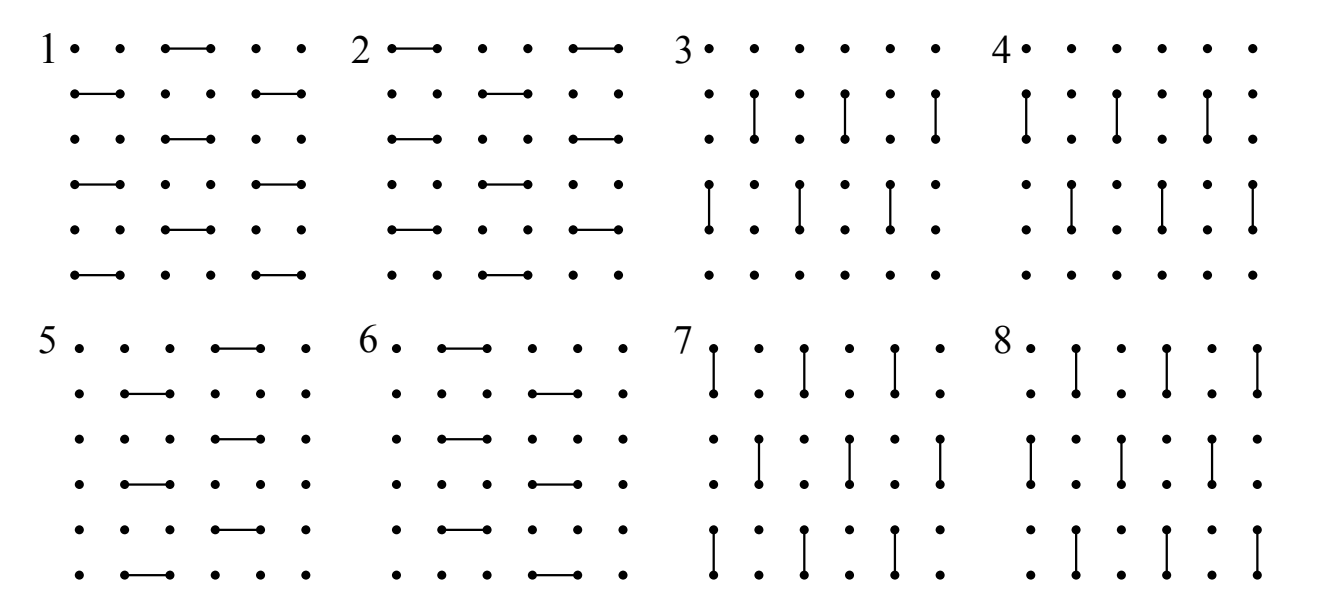
\includegraphics[width=0.58\textwidth]{figures/cz_order}
  \caption[Order of $CZ$ Gate Applications in Random Circuits]{Order (1 to 8) in which $CZ$ gates are applied to the qubits. As 
  the qubits are aligned on a 2D lattice, only neighboring qubits can be coupled through $CZ$ gates. 
  The pattern repeats every 8 cycles. Figure taken from \cite{Boixo2018supremacy}.}
  \label{fig:czgates}
\end{figure}

Boixo et al. were able to numerically show that the output distribution of random circuits generated this way
converge to Porter-Thomas after a square root
number of cycles in the number of qubits \cite{Boixo2018supremacy}.

\section{Experiments on the Sycamore Processor}
\label{sec:experiments_sycamore}

Built upon the theoretical framework of random circuit sampling,
a team from Google and the UCSB conducted a quantum
supremacy experiment on the 54 superconducting qubit \textit{Sycamore}
processor, shown in figure~\ref{fig:sycamore} \cite{martines2019supremacy}.

\begin{figure}[H]
  \centering
  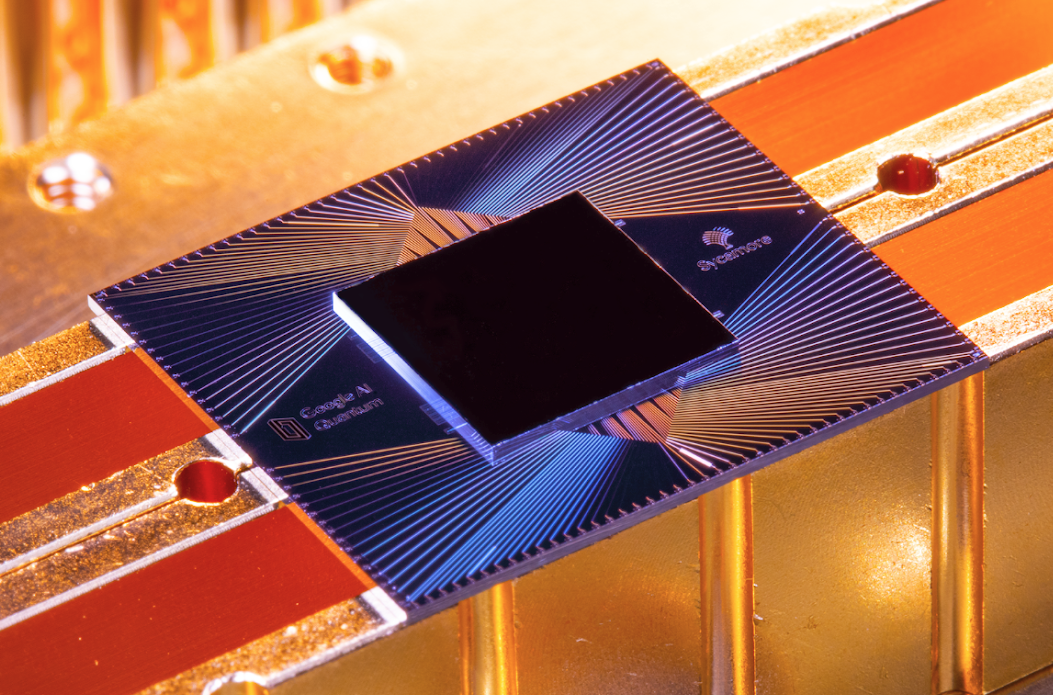
\includegraphics[width=0.58\textwidth]{figures/sycamore}
  \caption[The Sycamore Processor]{The Sycamore processor used in the quantum supremacy experiments of Google and UCSB. It consists of 54 qubits of which one was malfunctioning. Picture taken from \cite{martines2019supremacy}.}
  \label{fig:sycamore}
\end{figure}

For the experiments, they generated circuits with $n=10$ to $n=53$ qubits and
$m=12$ to $m=20$ cycles. The full cycles generated according to the procedure
given above can be classically simulated up to $n=53$ qubits with $m=14$ cycles
in a reasonable amount of time. Beyond that regime, simplified circuit
architectures, called \textit{elided} and \textit{patched}, were used. These circuits
are split into two sub-circuits with only weak entanglement in the elided and no
entanglement in the patched version. Such circuits can be classically simulated for up to $n=53$ qubits with $m=20$ cycles to
verify the fidelity of the Sycamore processor. For every setting of the circuit parameters, 20
circuits have been generated. For each circuit, $0.5-2.5$ million samples have been drawn
from the quantum processor \cite{martines2019supremacy}.

\begin{figure}[H]
  \centering
  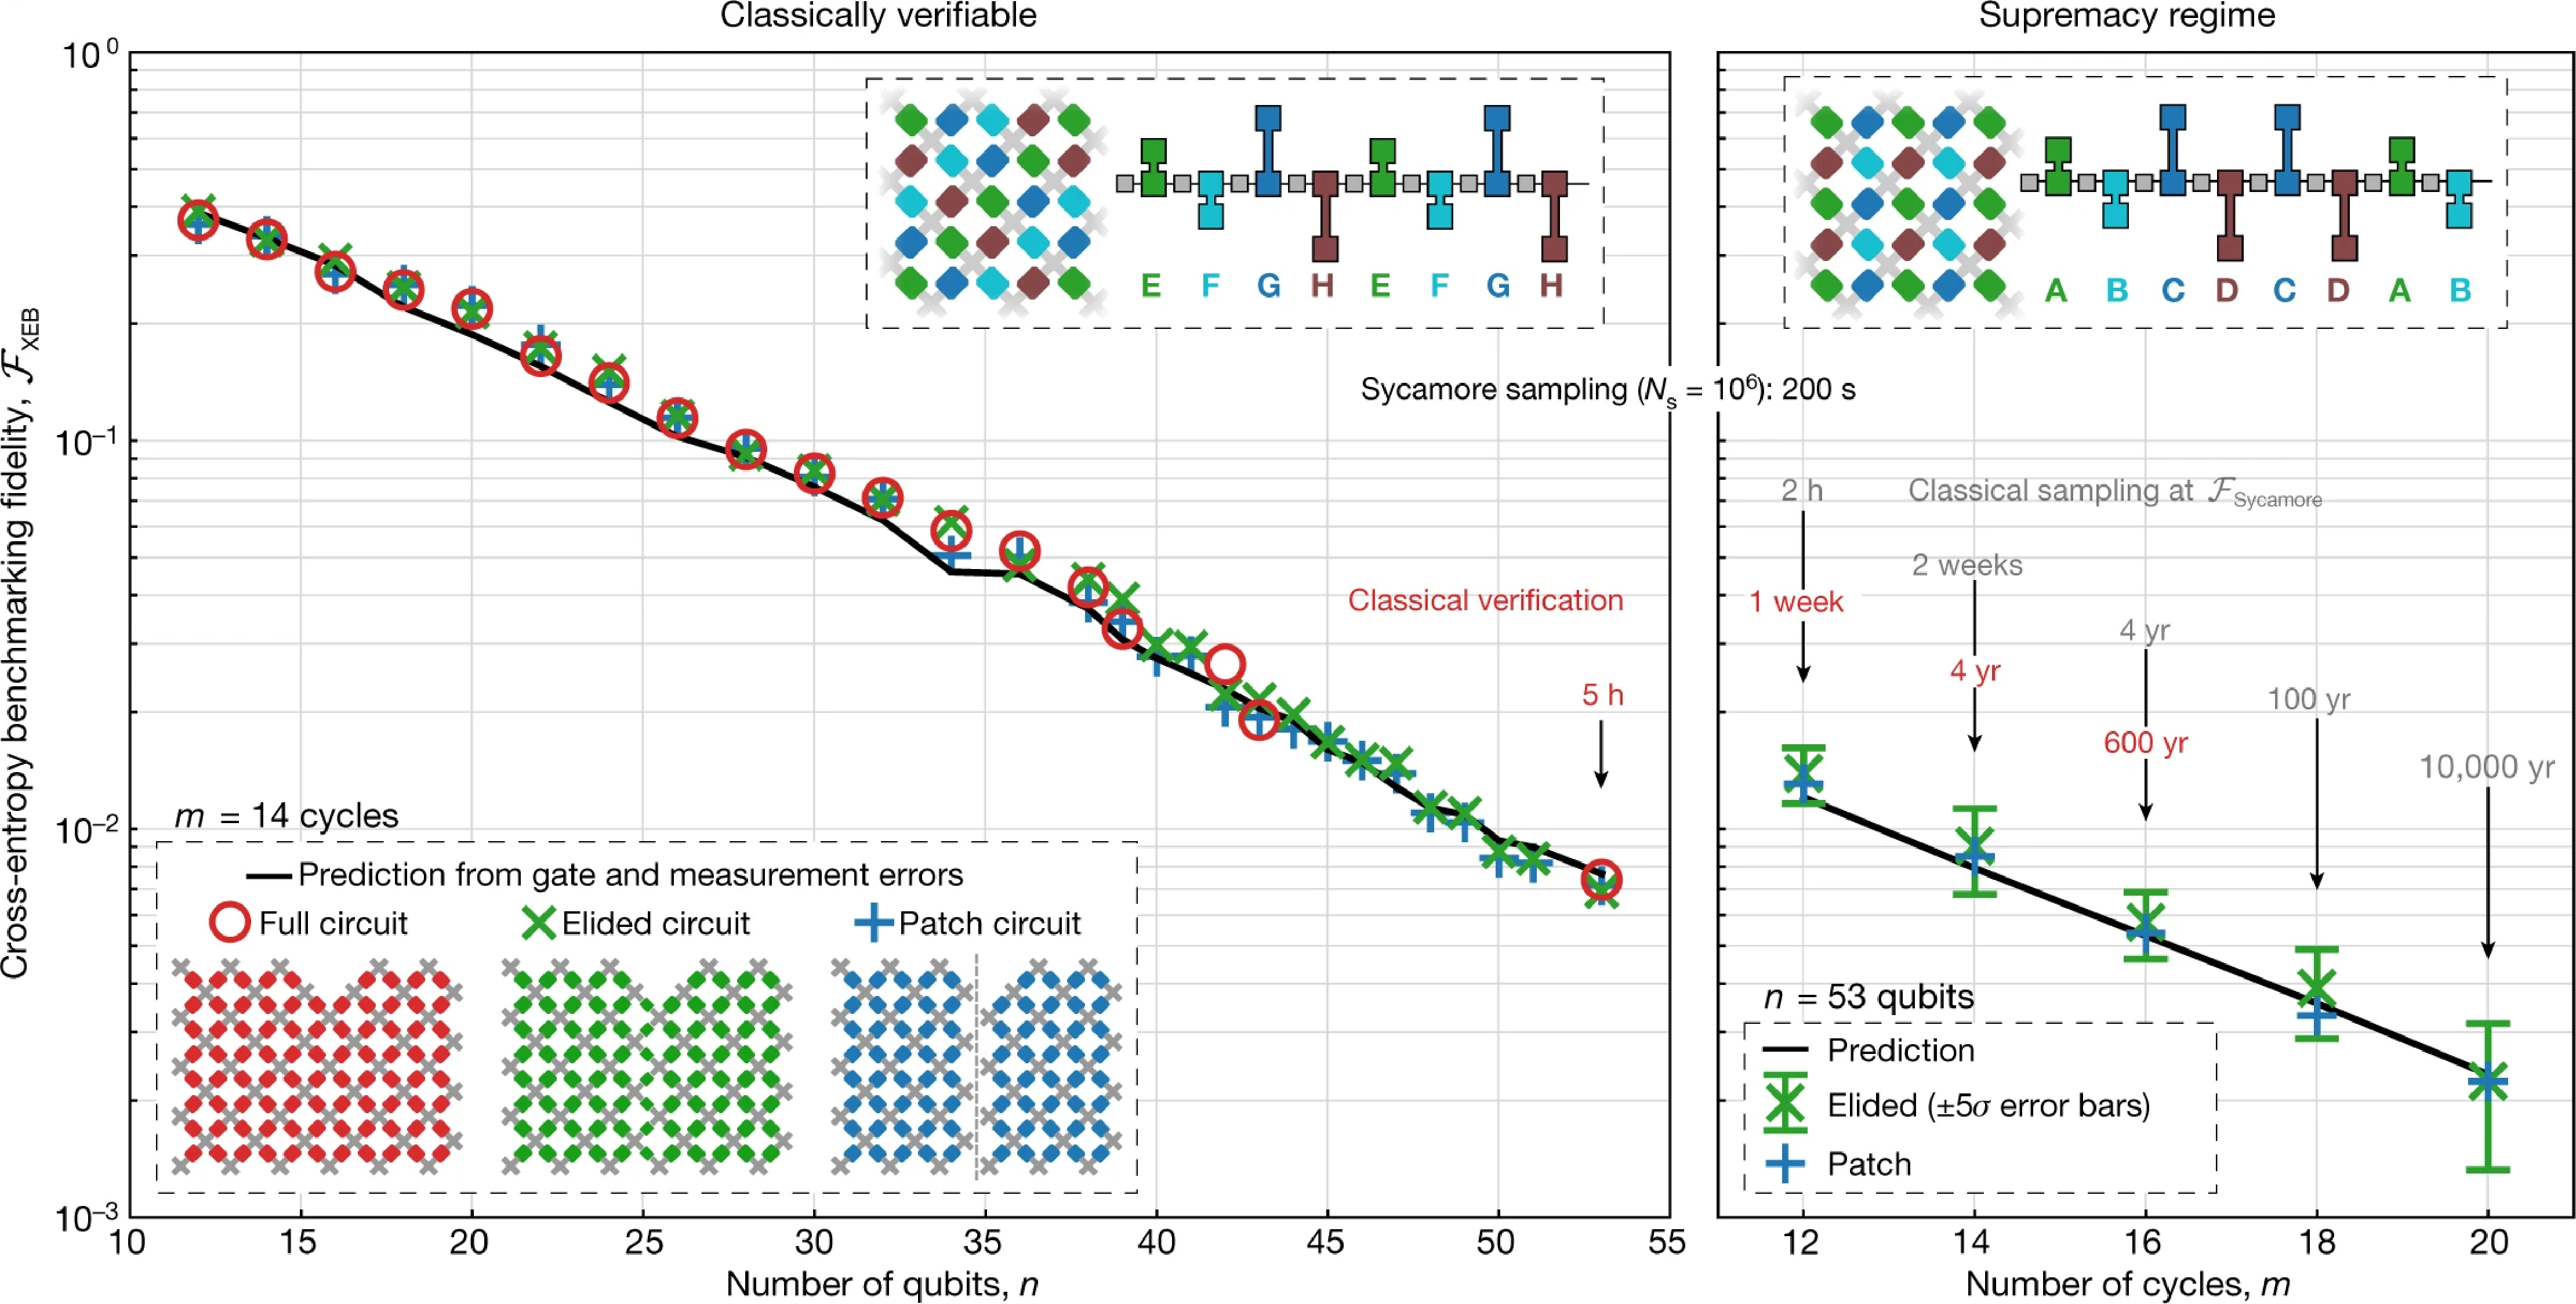
\includegraphics[width=\textwidth]{figures/supremacy_results}
  \caption[Cross Entropy Fidelity of the Sycamore Processor]{Results from the quantum supremacy experiments 
  with the Sycamore processor. The full circuits could only be simulated up to $n=53$ qubits and 
  $m=12$ cycles. Experiments on elided and patched circuits match the values of the extrapolated cross entropy difference.
  Figure taken from \cite{martines2019supremacy}.}
  \label{fig:supremacy_results}
\end{figure}

The team reports an average circuit fidelity $ > 0.1\%$ with $5\sigma$ confidence
for the largest elided circuits. All results fit the extrapolated expected
fidelity from smaller circuits, making the team conclude that similar fidelities
would be confirmed for the full circuits. As classical simulations of these
circuits would take up to 100,000 years according to the team with a hybrid
Schroedinger-Feynman algorithm, this would imply
that quantum supremacy has been achieved \cite{martines2019supremacy}. The reported fidelities of the quantum supremacy for
the different circuit sizes and depths are reported in figure~\ref{fig:supremacy_results}.

Shortly after these results have been announced, researchers from IBM claimed that the classical simulations
for the full circuits on 53 qubits and 20 cycles could have been performed
on the Summit supercomputer within a few days only with an optimized memory
usage \cite{pednault2019leveraging}. Experimental proof for these claims is still to be given.

Even if these circuits can be simulated within a few days, the quantum
processor would still outperform the classical simulation as it only
takes about 200ms to generate the 2 million samples for those circuits from it. As quantum
supremacy is a loosely defined term, the discussion might continue whether
quantum supremacy has been demonstrated by the Google and UCSB team. Nevertheless, 
the results prove that it is possible to build a quantum processor of 53 qubits
which can execute quantum circuits consisting of up to 1,113 single-qubit and
430 two-qubit gates with a single- and two-qubit gate fidelity greater than 99\% \cite{martines2019supremacy}.
For the future, the Google team expects a double exponential growth of the computational
power of quantum computers as the classical simulation costs grow exponentially
with the computational volume (gates and qubits) and quantum hardware
improvements will probably follow a quantum processor equivalent of Moore's law \cite{martines2019supremacy}.

This study does not focus on quantum circuits running on physical quantum devices,
but rather on the classical simulation. New and improved classical
approximate simulations of quantum systems with neural networks recently proved
to work well on many problem instances. 
Understanding their performance and necessary computational resources on
the RCS task might provide useful insights about the capabilities and
limitations of neural networks for the classical simulation of quantum systems.